\chapter{Funções}\label{cap:Funcoes}

\epigraph{``Nada que vale a pena é fácil''.}{Eric Cartman,  South Park}

\epigraph{``O ego é o pior inimigo do Eu, mas o Eu é o melhor amigo do ego... O ego é um péssimo senhor, mas é um ótimo servidor''.}{Bhagavad Gita}

\section{Conceitos, Definições e Nomenclaturas}\label{sec:FuncoesConceitoDefinicaoNomenclaturas}

Após o conceito importantíssimo de conjunto o componente mais importante na matemática é provavelmente a noção de função, o autor deste manuscrito não hesita em afirmar que você leitor com certeza já teve contato com a ideia de função, seja em seus curso do primário, secundário ou mesmo mais recentemente em suas disciplinas de nível superior tais como cálculo diferencial e integral ou alguma disciplina de física. 

Dado este encontra anterior do leitor sobre o assunto o autor fica confortável a pedir que leitor faça uma pequena pausa e tente lembrar de seus cursos anteriores e respondo para si mesmo ao questionamento: \textbf{o que é uma função}?

Bem, para muitos físicos, estatísticos e alguns matemáticos (não todos\footnote{Um visão interessante é aquela apontada em \cite{levin2021}, que descreve uma função como sendo um objeto com quatro descrições simultâneas: uma algébrica, uma numérica, uma gráfica e uma descritiva (ou em palavras).}), uma função é vista meramente como sendo um mapeamento (ou transformação) entre os elementos de dois conjuntos \cite{abe1991-TC}. Por outro lado, em obras tais como \cite{sussana2010-MD, lipschutz1971-Topo, lipschutz1978-TC, lipschutz2013-MD, Gerard2021discreta} uma função é vista como uma caso particular de relação entre dois conjuntos, ou seja, em última análise para esse grupo de pessoas uma função é exatamente um conjunto\footnote{Para melhor entender essa visão talvez o leitor deva revistar os Capítulos \ref{cap:Conjuntos} e \ref{cap:Relacoes} e revisar as definições apresentadas nos mesmo.}. Já em \cite{edward2019-MD, fmcbook} é apresentado uma visão mais mecanicista da ideia de função, essa visão captura a ideia de função enquanto uma máquina\footnote{Para cientistas da computação os termos máquina e programa são sinônimos.} (ou caixa preta) que transforma as entradas (\textit{inputs}) em saídas (\textit{outputs}), essa visão é ilustrada pela Figura \ref{fig:FuncaoBlackBox}. 

\begin{figure}[h]
	\centering
	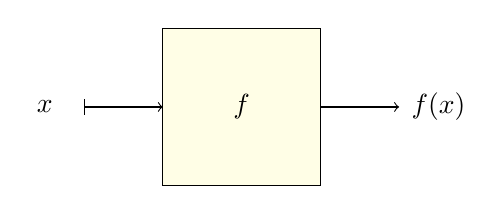
\begin{tikzpicture}
		\draw [rounded corners=0mm, fill=yellow!10]  (-1,1)--(-1,-1)--(1,-1)--(1,1)--cycle;
		\draw[->]  (1.0,0) -- (2.0,0.0);
		\draw[|->]  (-2.0,0) -- (-1.0,0.0);
		\node (f) at (0,0) {$f$};
		\node (fx) at (2.5,0) {$f(x)$};
		\node (x) at (-2.5,0) {$x$};
	\end{tikzpicture}
	\caption{Visão de uma função de uma variável enquanto uma máquina (ou caixa preta).}
	\label{fig:FuncaoBlackBox}
\end{figure}

Há também a ideia de função como sendo uma estrutura \cite{judith2021}, com componentes bem estabelecidos. Essa visão é capaz (como será mostrado a seguir) de captura todas as outras ideias de função.  Neste manuscrito a formalização da ideia de função como sendo uma estrutura será apresentada de forma gradual trançando paralelos com as linguagens de programação que possuam um sistema de tipos, isso será adotado para tornar o texto mais didático e interessante ao leitor de computação, além disso, irá aproximar os tópicos teóricos (as funções) dos tópicos práticos (programação) cujo leitor desse manuscrito naturalmente tem contato e provável interesse. Entretanto, esse forma de apresentação não será menos rigorosa que outras fontes bibliográficas, na verdade será o oposto, o texto aqui apresentado tende a ser mais preciso e detalhado que a apresentação rasa feita em \cite{judith2021}, por exemplo.

Este manuscrito irá iniciar o estudo sobre funções  apresentado ao leitor a ideia básica de assinatura de função, isto é, a seguir será apresentado a estrutura sintática que descreve as funções, ou seja, o componente descritivo mencionado em \cite{levin2021}.

\begin{definition}[Assinatura de Função]\label{def:AssinaturaFuncao}
	Sejam $A$ e $B$ conjuntos a assinatura da função de $A$ em $B$ nomeada como $f$ corresponde a uma palavra da forma $f: A \rightarrow B$.
\end{definition}

Note que a Definição \ref{def:AssinaturaFuncao} permite facilmente deduzir que em qualquer função existem três componentes básicos, sendo eles: um nome (rótulo ou símbolo funcional), um conjunto de partida e um conjunto de chegada. Por convenção, o nome de uma função deve ser sempre iniciado por caracteres latinos, no caso de usar índices apenas o último caractere do nome deve ser indexado.

\begin{example}\label{exe:AssinaturaFuncao}
	São exemplos de assinaturas de funções:
	\begin{itemize}
		\item[(a)] $g : \mathbb{N} \rightarrow \mathbb{Z}$.
		\item[(b)] $sqrt : \mathbb{R} \rightarrow \mathbb{R}$.
		\item[(c)] $k_1 : A \times B \rightarrow \mathbb{C}$.
		\item[(d)] $loc_2 : D \rightarrow \mathbb{R} \times \{0,1\}$.
		\item[(e)] $min : \mathbb{R}^n \rightarrow \mathbb{R}$.
		\item[(f)] $BUSCA : \mathbb{Z}^n \times \mathbb{Z} \rightarrow \{0,1\}$.
		\item[(g)] $BUSCA : \mathbb{R}^n \times \mathbb{R} \rightarrow \{0,1\}$.
	\end{itemize}
\end{example}

\begin{remark}
	O leitor deve observar que apesar das assinaturas nos itens (f) e (g) do Exemplo \ref{exe:AssinaturaFuncao} terem o mesmo nome, elas não são iguais, pois diferem no conjunto de partida, e assim não são a mesma assinatura. Esse tipo de cenário na computação recebe o nome de sobrecarga, isto é, o símbolo funcional $BUSCA$ está sobrecarregado para identificar duas funções distintas.
\end{remark}

Diversas linguagens de programação tais como C, C++ e Java apresentam a possibilidade de definir assinaturas de funções, na linguagem C por exemplo as assinaturas de funções que compõem uma biblioteca são geralmente reunidas em um arquivo de \textit{header}, isto é, um arquivo com a extensão .h, para mais detalhes consulte \cite{paulo2009algoritmos}, a seguir é exemplificado um arquivo de header.

\begin{figure}[h]
	\lstinputlisting[language=C]{codes/assinatura.h}
	\caption{Exemplo de um arquivo .h contendo assinaturas na linguagem C.}
	\label{fig:AssinaturasEmC}
\end{figure}

Um conceito indiretamente esboçado pela ideia de assinatura de função, é o de tipagem da função, sempre que a assinatura é da forma $f: A \rightarrow B$ pode-se dizer que $f$ é uma função do tipo ``$A$ em $B$'', ou mesmo que ``$f$ é um tipo seta de $A$ para $B$'', a noção de ``tipo seta'' é uma nomenclatura diretamente ligado a ideia de Teoria das categorias.

\begin{note}\label{note:TipoFuncao}
	Em geral programadores focados em linguagens imperativas tais como C (ou C++, Java e etc.) tende a erra a seguinte questão: ``Qual é o tipo da função reverse (definida na linha 2 da Figura \ref{fig:AssinaturasEmC})?'' A critério de esclarecimento tal função é do tipo seta de int em int, ou seja, matematicamente sua assinatura seria da forma, reverse: int $\rightarrow$ int.
\end{note}

Como dito anteriormente una função pode ser vista como uma máquina que transforma entradas em saídas, mas note que para que isso aconteça a máquina deve de alguma forma realizar ações sobre a entrada, ou seja, a máquina deve ``operar'' sobre a entrada. Esse conceito de como a máquina deve operar sobre as entradas é descrito por uma propriedade $P$ que define uma relação de mapeamento\footnote{Alguns textos usam a nomenclatura lei de formação, ver por exemplo \cite{carmo2013}.}

\begin{definition}[Relação de mapeamento]\label{def:RelacaoMapeamento}
	Dado dois conjuntos $A$ e $B$ e seja $x \in A$ e $y \in B$ a relação de mapeamento definida por uma propriedade $P$ corresponde  ao seguinte conjunto 
	$$\varepsilon = \{(x, y)\mid P\}$$ tal que $\varepsilon$ satisfaz a seguinte condição: se $(x, y_1), (x, y_2) \in \varepsilon$, então $y_1 = y_2$.
\end{definition}

Note que a Definição \ref{def:RelacaoMapeamento} apenas descreve que para cada entrada (variável) $x$ existirá uma única saída $y$ tal que $x$ e  $y$ estão relacionados por uma certa propriedade $P$.

\begin{example}\label{exe:RelacaoConstrucao}
	São exemplos de relações de mapeamento:
	\begin{itemize}
		\item[(a)] $\{(x, y) \in \mathbb{R}^2 \mid y = \log_2(x + 1)\}\}$
		\item[(b)] $\{(w_1w_2w_3\cdots w_m, y) \in E^2 \mid y = w_3\cdots w_mw_1w_2\}$ onde $E$ é o conjunto de todas as palavras do português com três letras ou mais e $w_i$ representa o $i$-ésimo símbolo de uma palavra $w$.
		\item[(c)] $\{(x, y) \in \mathbb{N}^2 \mid y = 14\}$.
		\item[(d)] $\Big\{(x_1, x_2, x_3, y) \in \mathbb{R} \times \mathbb{R} \times \mathbb{R}^*_+ \times \mathbb{R} \mid y = \sqrt[x_3]{\displaystyle\frac{1}{2}x_1 + x_2}\Big\}$.
	\end{itemize}
	Não são exemplos de relações de mapeamento:
	\begin{itemize}
		\item[(e)] $\{(x, y) \in N_P \times I_P\}$ onde $N_P$ é o conjunto de todos os nomes de pessoas e $I_P$ é o conjunto de naturais que representam idades, note que em tal relação é permitido que $(\text{Fátima}, 10), (\text{Fátima}, 55)$ estejam nesse conjunto, portanto, esse conjunto não satisfaz a Definição \ref{def:RelacaoMapeamento}.
		\item[(f)] $\{(x, y) \in \mathbb{R}  \mid \sqrt{y} = x\}$, note que $(5, 25)$ e $(-5, 25)$ pertence a tal conjunto e, portanto, esse conjunto não satisfaz a Definição \ref{def:RelacaoMapeamento}.
	\end{itemize}
\end{example}

\begin{remark}
	O item (c) do Exemplo \ref{exe:RelacaoConstrucao} é um caso interessante, a propriedade da relação descreve que para qualquer entrada $x$ a mesma sempre irá devolver como resposta um $y = 14$, ou seja, para todo $x$ tem-se que o par $(x, 14)$ está na relação. Esse tipo de relação de mapeamento será aqui chamada de \textbf{relação de mapeamento constante}.    
\end{remark}

Agora que foram apresentados estes conceitos fundamentais pode-se continuar o desenvolvimento deste texto com a formalização da ideia de função.

\begin{definition}[Função]
	Dado uma assinatura $f: A \rightarrow B$ e seja $\varepsilon \subseteq A \times B$ uma relação de mapeamento, a estrutura $\langle f: A \rightarrow B, \varepsilon \rangle$ é uma função.
\end{definition}

\begin{example}\label{exe:Funcoes}
	São exemplos de funções:
	\begin{itemize}
		\item[(a)] $\langle dob: \mathbb{N} \rightarrow  \mathbb{N},  \{(x, y) \in \mathbb{N}^2 \mid  y = 2x\} \rangle$.
		\item[(b)] $\langle mul: \mathbb{R} \times \mathbb{R} \rightarrow  \mathbb{N},  \{((x, y), z) \in \mathbb{R}^2 \times \mathbb{R} \mid  z = xy\} \rangle$.
		\item[(c)] $\langle sqroot: \mathbb{N} \rightarrow \mathbb{N},  \{(x, y) \in \mathbb{N}^2 \mid  y^2 = x\} \rangle$.
		\item[(d)] $\langle one: \mathbb{Z}^2 \rightarrow  \{1\},  \{((x, y), 1) \in \mathbb{Z}^2 \times \{1\} \mid  1 = x+y\} \rangle$.
		\item[(e)] $\langle sign: \mathbb{R} \rightarrow  \{0,1\},  \{(x, y) \in \mathbb{R} \times \{0, 1\} \mid y = 1 \text{ sempre que } x > 0.5 \text{ e } y = 0 \text{ se } x \leq 0.5\} \rangle$.
	\end{itemize}
\end{example}

De forma similar a apresentação feita em \cite{carmo2013} aqui será usado a própria relação de mapeamento para definir as noções de domínio e imagem de uma função.

\begin{definition}[Domínio e Imagem de função]\label{def:DomImaFuncao}
	Seja $\langle f: A \rightarrow B, \varepsilon \rangle$ uma função o domínio e a imagem de $f$, denotados respectivamente por $dom(f)$ e $ima(f)$, corresponde exatamente ao domínio e a imagem de $\varepsilon$, ou seja, $dom(f) = Dom(\varepsilon)$ e $ima(f) = Ima(\varepsilon)$.
\end{definition}

\begin{example}
	Considere a função $\langle k:\mathbb{R} \rightarrow \mathbb{R}, \{(x, y) \in \mathbb{R}^2 \mid y = \sqrt{x}\} \rangle$ tem-se que $dom(k) = ima(k) = \mathbb{R}^+$, pois claramente $(x, y) \in \varepsilon$ se, e somente se, $(x, y) = (x, \sqrt{x})$, agora obviamente $\sqrt{x}$ só existe para $x \geq 0$, logo $Dom(\varepsilon) = \mathbb{R}^+$, em contra partida para qualquer seja $\sqrt{x} \in \mathbb{R}$ tem-se que $\sqrt{x} \geq 0$, consequentemente, $Ima(\varepsilon) = \mathbb{R}^+$.
\end{example}

\begin{example}
	Considere a função $\langle prev:\mathbb{N} \rightarrow \mathbb{N}, \{(x, y) \in \mathbb{N}^2 \mid y = n - 1\} \rangle$, note que $(x, y) \in \varepsilon$ se, e somente se, $(x, y) = (x, x-1)$, mas $x - 1 \in \mathbb{N}$ apenas se $x > 0$, portanto,  tem-se que $dom(prev) = \mathbb{N}_*$. Por outro lado, para qualquer $x > 0$ tem-se que $x - 1 \in \mathbb{N}$ e, portanto, não é difícil verificar que  $Ima(\varepsilon) = \mathbb{N}$, consequentemente, $Ima(prev) = \mathbb{N}$.
\end{example}

Agora é comum ao estudar funções como destacado em \cite{carmo2013}, não ficar declarando a estrutura da função o tempo inteiro, em vez disso, em geral é descrita a assinatura da função junto com o açúcar sintático detalhado a seguir.

\begin{note}[Açúcar sintático]\label{def:acucarFuncao}
	Seja  $\langle f: A \rightarrow B, \varepsilon \rangle$ uma função, $f(x)$ é um açúcar sintático para dizer que $f$ está recebendo como entrada $x$, se escreve $f(x) = y$ como açúcar sintático da frase: ``ao calcular $f$ com entrada $x$ é gerado $y$ como saída'', mas para isso necessário que $(x, y) \in \varepsilon$. Agora observe que quando a relação $\varepsilon$ de uma função descreve $y$ a partir de uma igualdade da forma $y = E$, em que $E$ é uma expressão válida, pode-se em vez de, fazer $f(x) = y$ escreve diretamente $f(x) = E$, e desde que $y = E$ a expressão $f(x) = E$ é um refinamento do açúcar sintático.
\end{note}

\begin{example}
	Usando as ideias do açúcar sintático descrito na Nota \ref{def:acucarFuncao} tem-se que:
	\begin{itemize}
		\item[(a)] A função  $\langle dob: \mathbb{N} \rightarrow  \mathbb{N},  \{(x, y) \in \mathbb{N}^2 \mid  y = 2x\} \rangle$ pode simplesmente ser escrita usando sua assinatura $dob:\mathbb{N} \rightarrow  \mathbb{N}$ e dizendo que $dob(x) = 2x$.
		\item[(b)] A função  $\langle pot: \mathbb{R} \times \mathbb{N} \rightarrow  \mathbb{R},  \{((x, y), z) \in (\mathbb{R} \times \mathbb{N}) \times \mathbb{R} \mid  z = x^y\} \rangle$ pode simplesmente ser escrita usando sua assinatura $pot: \mathbb{R} \times \mathbb{N} \rightarrow  \mathbb{R}$ e dizendo que $pot(x, y) = x^y$.
	\end{itemize}
\end{example}

\begin{remark}
	Deste ponto em diante sempre que for possível será usado apenas a assinatura para se referir a uma função.
\end{remark}

Note que se $f$ é uma função com assinatura $f: A \rightarrow B$, isto é, $f$ é um objeto do tipo seta de $A$ em $B$, e $x$ um objeto do tipo $A$\footnote{Em teoria dos tipos \cite{nederpelt2014, thompson1999} se $A$ é um tipo e $x$ é um objeto do tipo $A$ pode-se escrever que $x:A$, isto é algo semelhante a teoria dos conjuntos ao dizer que $x \in A$.} pode-se pensar em uma regra capaz de deduzir o tipo da saída de $f(x)$, tal regra poderia ser nomeada como $iType$ e poderia ser escrita como:
\begin{equation*}
	\infer[iType]{f(x):B}{x:A & f:A \rightarrow B}
\end{equation*}
essa regra não é algo novo criado nesse manuscrito, na verdade a mesma em um certo ponto de vista é uma versão da famosa regra de \textit{modus ponens} (ver Capítulo \ref{cap:LogicaProposicional}), a existência de tal regra é uma manifestação da profunda conexão que existe entre lógica e computação. Tal conexão é conhecida como isomorfismo de Curry–Howard, e é um aspecto fundamental em áreas como teoria dos tipos \cite{nederpelt2014, thompson1999}, teoria da prova \cite{nederpelt2014, sergey2014}, $\lambda$-cálculo \cite{bare1984, henk1992, bimbo2019} e programação funcional \cite{thompson1999, fmcbook}.

\begin{figure}[h]
	\lstinputlisting[language=C]{codes/sqfunction.c}
	\caption{Código da implementação da função no item (c) do Exemplo \ref{exe:Funcoes} escrito na linguagem C.}
	\label{fig:FuncaoSqrt}
\end{figure}

Agora note que a Definição \ref{def:DomImaFuncao} não impõe de forma alguma que todos os elementos do conjunto de partida de uma função estejam no seu domínio, e isso gera situação interessantes tanto do ponto de vista teórico quando do ponto de vista prático, para ilustra essa questão considere o código fonte na linguagem C esboçado na Figura \ref{fig:FuncaoSqrt} que implementa a função (c) do Exemplo \ref{exe:Funcoes} , o que ocorre se tal código receber como entrada um $x$ com valor $3$? Bem para um programador com um pouco de experiência nota facilmente que o algoritmo não retorna nada, ficando em \textit{loop} eterno\footnote{Um simples teste de mesa pode mostra a verdade dessa afirmação, para saber mais sobre testes de mesa ver \cite{medina2006}.}. Para entender essa resposta deve-se atentar aos seguintes fatos:

\begin{enumerate}
	\item O fato principal é que $\sqrt{3} \notin \mathbb{N}$, ou seja, não existe um $y \in \mathbb{N}$ tal que $y = \sqrt{3}$.
	\item A partir do item anterior é claro que não existe um par $(x, y)$ na relação definida pela propriedade $y = \sqrt{x}$ quando $x = 3$.	
\end{enumerate}

Assim a função $sqrt$ definida no item (c) do Exemplo \ref{exe:Funcoes} não pode produzir uma saída para a entrada $x = 3$. Do ponto de vista prático (implementação) o programa acima encerra e retorna um $y$ como saída se, e somente se,  $y = \sqrt{x} \in \mathbb{N}$, dessa forma pode-se pensar que a noção da divergência (ou \textit{loop} eterno) de programas pode ser usada para modelar a indefinição de funções, isto é, quando um programa $prog$ é a implementação de um função $f$ sempre que $prog$ receber uma entrada para a qual $f$ não calcula uma saída o programa $prog$ fica em divergência.

Considerando essa pequena discussão pode-se então pensar em separar (ou tipar) as funções, as funções que estão definidas para todas as entradas e as funções que não estão definidas para todas as entradas, essa tipagem é formalizada na definição que se segue.

\begin{definition}[Funções totais e parciais]
	Uma função $f: A \rightarrow B$ é dita ser total sempre que $dom(f) = A$ e será dita parcial sempre que $dom(f) \subseteq A$.
\end{definition}

\begin{example}\label{exem:FuncoesTotaisParciais1}
	Considerando as assinaturas $f: \mathbb{Z} \rightarrow \mathbb{Z}$, $g, h: \mathbb{N} \rightarrow \mathbb{N}$ e $i: \mathbb{R} \rightarrow \mathbb{R}_+$ tem-se que:
	\begin{itemize}
		\item[(a)] $f(x) = x - 1$ é uma função total. 
		\item[(b)] $g(x) = \frac{1}{x}$ é uma função parcial, visto que $\frac{1}{0} \notin \mathbb{N}$.
		\item[(c)] $h(x) = x^2 + 3$ é uma função total.
		\item[(d)] $i(x) = x - 5$ é uma função parcial, pois tem-se que $1 - 5 = -4$ e $-4 \notin \mathbb{R}_+$.
	\end{itemize}
\end{example}

\begin{example}\label{exem:FuncoesTotaisParciais2}
	Seja $List_{int}$ o conjunto de todas as lista de $int$ da linguagem C, tem-se que a função $first_{int}$ que recebe uma lista de $int$ e retorna o primeiro elemento da mesma não é uma função total, pois se a mesma receber a lista vazia não há um primeiro elemento a ser retornado e assim a mesma deve entrar em divergência.
\end{example}

\begin{remark}
	O leitor deve observar que a assinatura de uma função é capaz de mudar seu tipo totalmente, por exemplo, a função $f$ do Exemplo \ref{exem:FuncoesTotaisParciais1} com a assinatura $f: \mathbb{N} \rightarrow \mathbb{N}$ passa a ser uma função parcial.
\end{remark}

Um ponto interessante que talvez o leitor tenha percebido no Exemplo \ref{exem:FuncoesTotaisParciais1} é que, para mostrar a parcialidade de uma função basta apresentar um elemento do conjunto de partida para o qual a função em questão não está definida, dessa forma o conjunto de partida é diferente do domínio da função e, portanto, a função é parcial. A seguir é apresentado a definição do espaço de função, um conceito que será importante no decorrer deste manuscrito.

\begin{definition}[Conjunto ou Espaço de Funções]
	Sejam $A$ e $B$ conjuntos (não necessariamente distintos), o conjunto ou espaço de todas as funções de $A$ em $B$ é denotado por $B^A$\footnote{Também é encontrado na literatura o uso de $(f: A \rightarrow B)$ para denotar o espaço de função \cite{fmcbook}.}.
\end{definition}